\documentclass[12pt,a4paper]{article}

\usepackage[utf8]{inputenc}
\usepackage[T1]{fontenc}
\usepackage[english]{babel}
\usepackage[margin=2.5cm]{geometry}
\usepackage{hyperref}
\usepackage{xcolor}
\usepackage{longtable}
\usepackage{booktabs}
\usepackage{array}
\usepackage{enumitem}
\usepackage{titlesec}
\usepackage{fancyhdr}
\usepackage{multirow}
\usepackage{tabularx}
\usepackage{colortbl}
\usepackage{tikz}
\usepackage{pgf-umlcd}
\usetikzlibrary{shapes,arrows.meta,positioning,fit,backgrounds,calc}

\definecolor{vinotinto}{HTML}{8D191D}
\definecolor{ocre}{HTML}{D8CEA3}
\definecolor{grisusco}{HTML}{4E6470}
\definecolor{softblue}{HTML}{D6E4F0}
\definecolor{softgreen}{HTML}{D5F5E3}
\definecolor{softyellow}{HTML}{FDEBD0}

\titleformat{\section}{\large\bfseries\color{vinotinto}}{\thesection}{1em}{}[\titlerule]
\titleformat{\subsection}{\normalsize\bfseries\color{grisusco}}{\thesubsection}{1em}{}

\pagestyle{fancy}
\fancyhf{}
\fancyhead[L]{\small\color{grisusco}SIPAM-USCO — AI Course Project}
\fancyhead[R]{\small\color{grisusco}Technical Documentation v1.0}
\fancyfoot[C]{\thepage}
\renewcommand{\headrulewidth}{0.4pt}

\newcommand{\method}[1]{\texttt{\textbf{\color{vinotinto}#1}}}
\newcommand{\ep}[1]{\texttt{\color{grisusco}#1}}
\newcommand{\role}[1]{\textit{\color{vinotinto}#1}}

% ─────────────────────────────────────────────────────────────────────────────
\begin{document}

% ── Portada ──────────────────────────────────────────────────────────────────
\begin{titlepage}
  \centering
  \vspace*{1.5cm}
  {\color{vinotinto}\rule{\linewidth}{1.5pt}}\\[0.4cm]
  {\Huge\bfseries\color{vinotinto} SIPAM-USCO}\\[0.3cm]
  {\large Academic Internships and Tutoring Information System}\\[0.2cm]
  {\color{vinotinto}\rule{\linewidth}{1.5pt}}\\[0.8cm]
  {\LARGE\bfseries Technical Documentation}\\[0.4cm]
  {\large Artificial Intelligence Course Project — BEINSOF52}\\[1.8cm]
  \begin{tabular}{rl}
    \textbf{University:}    & Universidad Surcolombiana (USCO) \\[0.3cm]
    \textbf{Program:}       & Software Engineering \\[0.3cm]
    \textbf{Course:}        & Artificial Intelligence (BEINSOF52) \\[0.3cm]
    \textbf{Professor:}     & Juan Antonio Castro Silva \\[0.3cm]
    \textbf{Version:}       & 1.0.0 \\[0.3cm]
    \textbf{Stack:}         & FastAPI · Flask · PostgreSQL · React · TensorFlow \\[0.3cm]
    \textbf{Date:}          & May 2026 \\
  \end{tabular}
  \vfill
  {\color{grisusco}\small Document generated from source code — SIPAM-USCO v1.0}
\end{titlepage}

\tableofcontents
\newpage

% ══════════════════════════════════════════════════════════════════════════════
\section{Introduction}
% ══════════════════════════════════════════════════════════════════════════════

\textbf{SIPAM-USCO} (Sistema de Información de Prácticas Académicas y Monitorías) is a
full-stack web application developed as a thesis project for the Software Engineering program at
the Universidad Surcolombiana. The system digitizes and automates two critical academic
administrative processes that were previously handled entirely on paper.

The system manages:
\begin{itemize}
  \item \textbf{Academic Tutoring (Monitorías):} Full lifecycle management of monitor
        recruitment, selection, hour tracking, and performance evaluation.
  \item \textbf{Field Practices (Prácticas Extramuros):} Multi-stage approval workflow for
        out-of-campus academic field trips, including budget management, transport cost
        calculation, consent form collection, and institutional PDF form generation.
  \item \textbf{AI-Powered Monitor Selection Predictor:} A machine learning microservice
        (Flask + TensorFlow) that predicts the probability of a student being selected as a
        monitor, integrated with the main system.
\end{itemize}

The system serves five user roles: \role{estudiante} (student), \role{profesor} (professor),
\role{jefe\_programa} (program director), \role{decano} (dean), and \role{admin}
(administrator/vice-rector).

% ══════════════════════════════════════════════════════════════════════════════
\section{Problem Statement}
% ══════════════════════════════════════════════════════════════════════════════

The Faculty of Engineering at USCO currently manages academic tutoring and field practices
through paper-based processes and informal communication channels (email, WhatsApp). This
creates the following problems:

\begin{enumerate}
  \item \textbf{Lack of traceability:} No systematic record of application statuses, approval
        decisions, or state transitions.
  \item \textbf{Manual selection:} Monitor candidates are evaluated manually, leading to
        inconsistencies and potential bias in the selection process.
  \item \textbf{Document overhead:} Each field practice requires the manual completion of
        institutional forms (FO-05, FO-15, FO-16, FO-46, FO-14), wasting significant time.
  \item \textbf{Budget opacity:} No integrated tool to track committed and executed budgets for
        transport and per-diem expenses.
  \item \textbf{Compliance risk:} Institutional agreements (Acuerdo 003/2012 and Acuerdo
        012/2023) define specific rules (minimum advance notice, maximum duration, quorum
        thresholds) that are hard to enforce manually.
\end{enumerate}

% ══════════════════════════════════════════════════════════════════════════════
\section{Objectives}
% ══════════════════════════════════════════════════════════════════════════════

\subsection*{General Objective}
To design and implement an intelligent information system that automates the management of
academic tutoring and field practices at USCO, incorporating an AI-based prediction module for
monitor candidate selection.

\subsection*{Specific Objectives}
\begin{enumerate}
  \item Implement a digital workflow for the three-stage approval process of field practices
        according to Acuerdo 003/2012.
  \item Automate the weighted selection algorithm (RF-MON-05) for monitor candidates, with
        a machine learning model to predict selection outcomes.
  \item Generate institutional PDF forms automatically from stored data.
  \item Build a budget management module tracking committed, executed, and available funds.
  \item Provide real-time transport cost estimation using INVIAS toll data and SICOM fuel
        price feeds.
  \item Deploy a Flask-based AI microservice exposing a REST API for selection prediction,
        trained on SIPAM's PostgreSQL data.
  \item Deliver a responsive React frontend that integrates all system features including the
        AI predictor interface.
\end{enumerate}

% ══════════════════════════════════════════════════════════════════════════════
\section{State of the Art}
% ══════════════════════════════════════════════════════════════════════════════

\subsection{Academic Information Systems}
University management systems such as Banner, Ellucian, and SAP Student Lifecycle Management
provide general academic administration but lack context-specific workflows for Colombian
institutional regulations. Regional systems at Colombian universities (UNAL SIA, UIS SIRA)
handle enrollment but do not address the specific needs of the Acuerdo 003/2012 approval
pipeline or the Acuerdo 012/2023 tutoring framework.

\subsection{Machine Learning for Student Performance Prediction}
Several studies have applied machine learning to predict academic outcomes:
\begin{itemize}
  \item \textbf{Romero \& Ventura (2020):} Surveyed educational data mining techniques,
        highlighting Random Forest and gradient boosting as top performers for classification
        tasks in academic contexts.
  \item \textbf{Hussain et al. (2018):} Used decision trees and SVM to predict student
        performance, achieving 85\% accuracy on dropout prediction.
  \item \textbf{Mduma et al. (2019):} Applied ensemble methods (bagging, boosting) for
        student retention prediction in African universities.
\end{itemize}

Our approach adapts these techniques to the specific task of monitor selection prediction,
using academic features (GPA, credit completion rate, subject grade, interview score) to
classify candidates as likely selected or not.

\subsection{Microservice Architectures for AI Integration}
The Flask microservice pattern for AI inference is well established:
\begin{itemize}
  \item \textbf{Sculley et al. (2015)} — "Hidden Technical Debt in Machine Learning Systems"
        advocates separating training and inference pipelines.
  \item \textbf{Amershi et al. (2019)} — Software engineering best practices for ML systems
        emphasize model versioning and API-based deployment.
\end{itemize}

% ══════════════════════════════════════════════════════════════════════════════
\section{Requirements}
% ══════════════════════════════════════════════════════════════════════════════

\subsection{Functional Requirements}
\begin{longtable}{>{\bfseries}p{2.5cm} p{5cm} p{5.5cm}}
  \toprule
  \textbf{ID} & \textbf{Name} & \textbf{Description} \\
  \midrule
  \endfirsthead
  \toprule \textbf{ID} & \textbf{Name} & \textbf{Description} \\ \midrule \endhead
  RF-MON-01 & Academic validation & Verify GPA $\geq$ 3.50 and credits $\geq$ 30\% \\
  RF-MON-02 & Application & Apply with documents within the open period \\
  RF-MON-03 & Document upload & Upload and download supporting documents \\
  RF-MON-04 & Academic evaluation & Record subject grade and interview score \\
  RF-MON-05 & Selection algorithm & Weighted 30/30/40 selection with tiebreaker \\
  RF-MON-06 & Hour tracking & Weekly hour log by monitor (weeks 1–20) \\
  RF-MON-07 & Hour approval & Professor approves logged hours \\
  RF-MON-08 & Performance evaluation & Final monitor evaluation by professor \\
  RF-MON-09 & Disciplinary sanction & Block application if sanctioned (Art.4.c) \\
  RF-MON-10 & Withdrawal & Voluntary withdrawal from application \\
  RF-AI-01  & Selection prediction & ML model predicts selection probability \\
  RF-PRA-01 & Practice request & Create with route, dates, and FO-16 data \\
  RF-PRA-02 & Minimum advance & Request $\geq$ 30 days before start \\
  RF-PRA-03 & Duration limit & 3 days (Huila) / 4 days (outside Huila) \\
  RF-PRA-04 & Approval flow & Three stages: curriculum, faculty, vice-rector \\
  RF-PRA-05 & Rejection & Stage-based rejection with observations \\
  RF-PRA-06 & Consent window & Opens D-10, closes D-5 \\
  RF-PRA-07 & Digital signature & Digital consent with IP and timestamp \\
  RF-PRA-08 & Auto quorum & Auto-advance at 66\% signatures \\
  RF-PRA-09 & Per-diem calculation & Based on current rates and duration \\
  \bottomrule
\end{longtable}

\subsection{Non-Functional Requirements}
\begin{longtable}{>{\bfseries}p{2.5cm} p{4cm} p{6cm}}
  \toprule
  \textbf{ID} & \textbf{Name} & \textbf{Description} \\
  \midrule
  RNF-01 & JWT Auth & Secure tokens with configurable expiry \\
  RNF-02 & Role-based access & Granular permissions per endpoint \\
  RNF-03 & Brute-force protection & 5 attempts / 15 min, persisted in DB \\
  RNF-04 & Audit trail & Critical actions logged in audit\_logs \\
  RNF-05 & File security & MIME type and extension validation \\
  RNF-06 & HTTP security headers & CSP, X-Frame-Options, HSTS \\
  RNF-07 & DB integrity & CHECK constraints on all critical ranges \\
  RNF-08 & DB performance & Indexes on all frequently filtered columns \\
  RNF-09 & ML reproducibility & Fixed random seeds, 70-15-15 split \\
  RNF-10 & Model serialization & Trained model persisted as .joblib/.h5 \\
  \bottomrule
\end{longtable}

% ══════════════════════════════════════════════════════════════════════════════
\section{User Stories}
% ══════════════════════════════════════════════════════════════════════════════

\begin{longtable}{>{\bfseries}p{1.2cm} p{2.5cm} p{9.3cm}}
  \toprule
  \textbf{ID} & \textbf{Role} & \textbf{Story} \\
  \midrule
  \endfirsthead
  \toprule \textbf{ID} & \textbf{Role} & \textbf{Story} \\ \midrule \endhead

  HU-01 & Professor & \textbf{As} a professor, \textbf{I want} to create a tutoring vacancy for a specific subject, \textbf{so that} I can find qualified students to support the course. \\[4pt]
  HU-02 & Student & \textbf{As} a student, \textbf{I want} to apply for a tutoring position with supporting documents, \textbf{so that} I can participate in the selection process. \\[4pt]
  HU-03 & Student & \textbf{As} a student, \textbf{I want} to withdraw my application before selection, \textbf{so that} I have control over my participation. \\[4pt]
  HU-04 & Professor & \textbf{As} a professor, \textbf{I want} to register subject grades and interview scores per applicant, \textbf{so that} the selection algorithm has all required data. \\[4pt]
  HU-05 & Prof / Head & \textbf{As} a professor, \textbf{I want} to run the weighted selection algorithm, \textbf{so that} I get an objective ranked list of candidates. \\[4pt]
  HU-06 & Student & \textbf{As} a selected monitor, \textbf{I want} to log my weekly hours, \textbf{so that} the system tracks my service fulfillment. \\[4pt]
  HU-07 & Professor & \textbf{As} a professor, \textbf{I want} to approve my monitors' logged hours weekly, \textbf{so that} I can validate contract compliance. \\[4pt]
  HU-08 & Student & \textbf{As} a student, \textbf{I want} to see my predicted probability of being selected before applying, \textbf{so that} I can make an informed decision. \\[4pt]
  HU-09 & Professor & \textbf{As} a professor, \textbf{I want} to create a field practice request with route details and justification, \textbf{so that} I can initiate the institutional approval process. \\[4pt]
  HU-10 & Student & \textbf{As} a student, \textbf{I want} to digitally sign the informed consent form, \textbf{so that} I can confirm my voluntary participation. \\[4pt]
  HU-11 & Head & \textbf{As} a program director, \textbf{I want} to approve or reject practices at the curriculum committee stage, \textbf{so that} I ensure academic relevance of field trips. \\[4pt]
  HU-12 & Admin & \textbf{As} an administrator, \textbf{I want} to manage the semester budget and see committed vs.\ executed amounts, \textbf{so that} I control institutional spending. \\[4pt]
  \bottomrule
\end{longtable}

% ══════════════════════════════════════════════════════════════════════════════
\section{Use Case Diagrams}
% ══════════════════════════════════════════════════════════════════════════════

\subsection{Tutoring Module — Use Cases}

\begin{center}
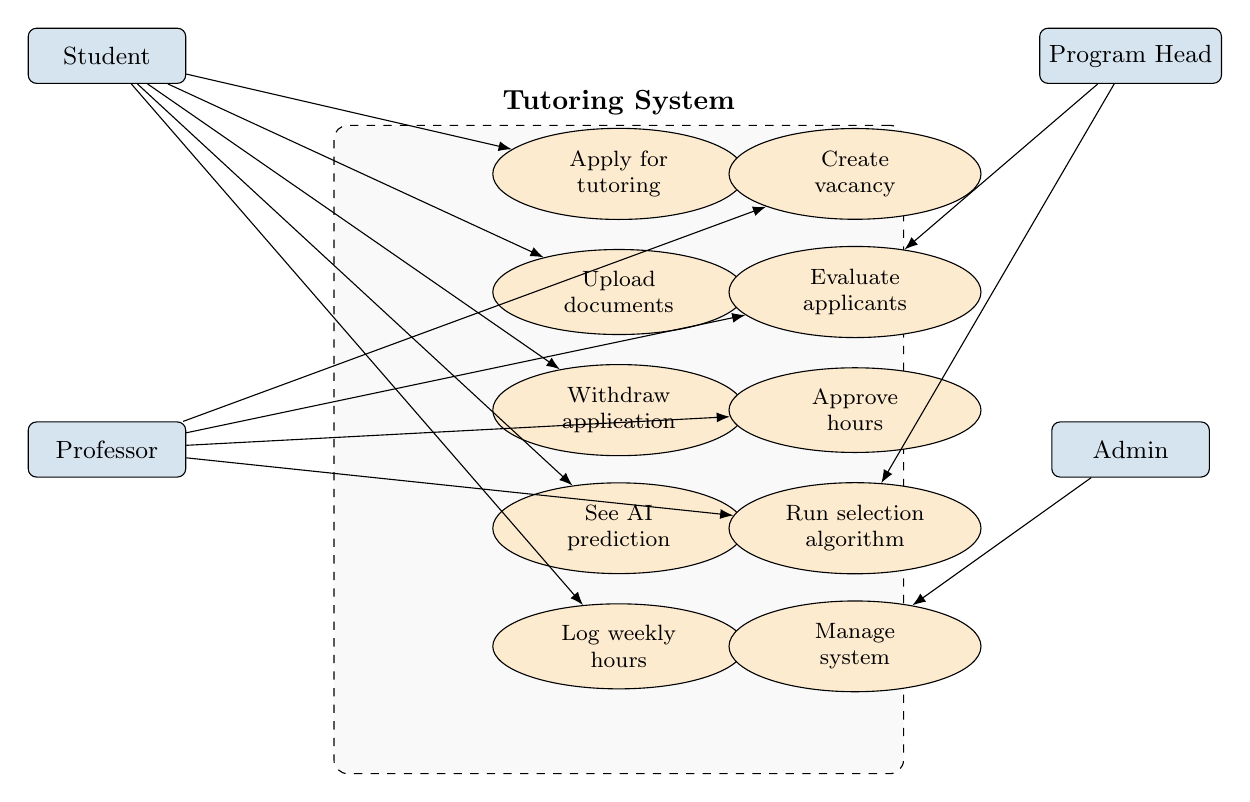
\begin{tikzpicture}[
  actor/.style={draw, rectangle, rounded corners=3pt, minimum width=2cm, minimum height=0.7cm, fill=softblue, font=\small},
  usecase/.style={draw, ellipse, minimum width=3.2cm, minimum height=0.7cm, fill=softyellow, font=\footnotesize, align=center},
  system/.style={draw, dashed, rectangle, rounded corners=5pt, fill=gray!5},
  arr/.style={->, >=Latex, thin}
]
  \node[actor] (student) at (0,0) {Student};
  \node[actor] (prof) at (0,-5) {Professor};
  \node[actor] (jefe) at (13,0) {Program Head};
  \node[actor] (admin) at (13,-5) {Admin};

  \begin{scope}[on background layer]
    \node[system, fit={(3,-1)(10,-9)}, label=above:{\textbf{Tutoring System}}] {};
  \end{scope}

  \node[usecase] (apply)   at (6.5,-1.5) {Apply for\\tutoring};
  \node[usecase] (upload)  at (6.5,-3.0) {Upload\\documents};
  \node[usecase] (withdraw)at (6.5,-4.5) {Withdraw\\application};
  \node[usecase] (predict) at (6.5,-6.0) {See AI\\prediction};
  \node[usecase] (loghours)at (6.5,-7.5) {Log weekly\\hours};
  \node[usecase] (create)  at (9.5,-1.5) {Create\\vacancy};
  \node[usecase] (evaluate)at (9.5,-3.0) {Evaluate\\applicants};
  \node[usecase] (approve) at (9.5,-4.5) {Approve\\hours};
  \node[usecase] (runalgo) at (9.5,-6.0) {Run selection\\algorithm};
  \node[usecase] (manage)  at (9.5,-7.5) {Manage\\system};

  \draw[arr] (student) -- (apply);
  \draw[arr] (student) -- (upload);
  \draw[arr] (student) -- (withdraw);
  \draw[arr] (student) -- (predict);
  \draw[arr] (student) -- (loghours);
  \draw[arr] (prof) -- (create);
  \draw[arr] (prof) -- (evaluate);
  \draw[arr] (prof) -- (approve);
  \draw[arr] (prof) -- (runalgo);
  \draw[arr] (jefe) -- (runalgo);
  \draw[arr] (jefe) -- (evaluate);
  \draw[arr] (admin) -- (manage);
\end{tikzpicture}
\end{center}

\subsection{Field Practices Module — Use Cases}

\begin{center}
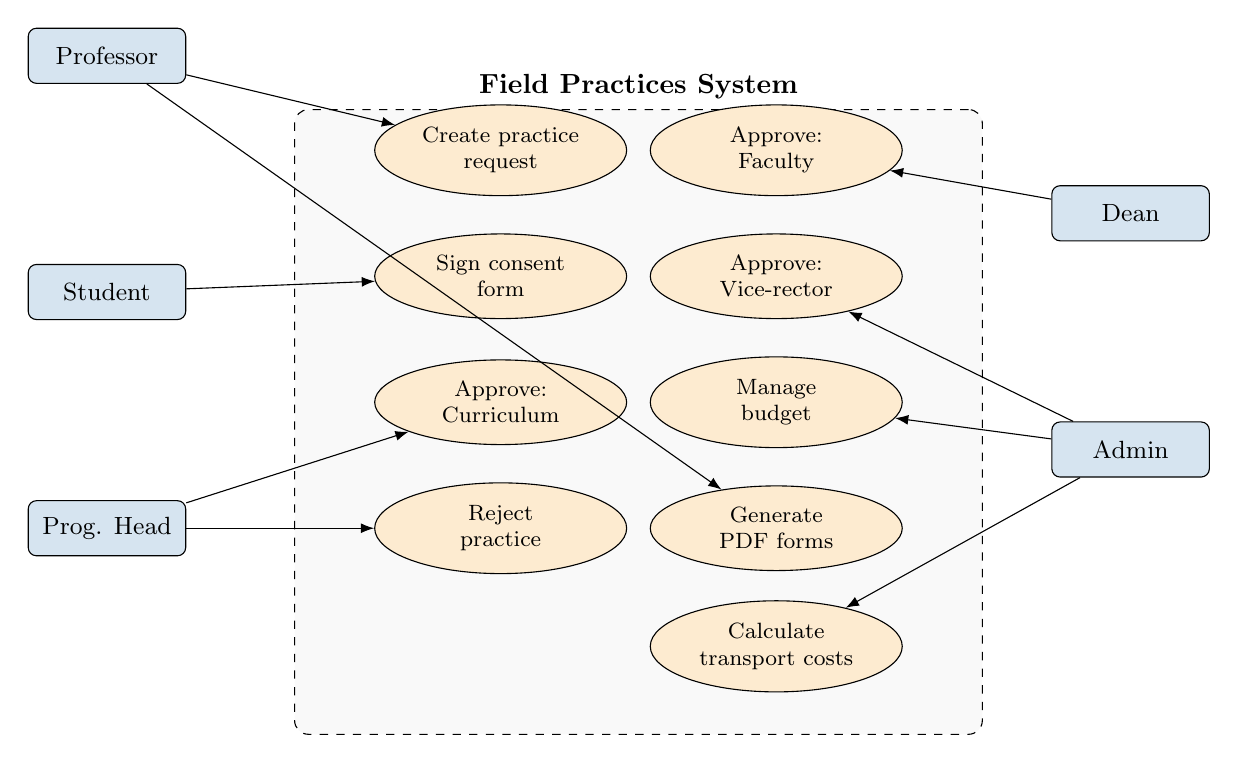
\begin{tikzpicture}[
  actor/.style={draw, rectangle, rounded corners=3pt, minimum width=2cm, minimum height=0.7cm, fill=softblue, font=\small},
  usecase/.style={draw, ellipse, minimum width=3.2cm, minimum height=0.7cm, fill=softyellow, font=\footnotesize, align=center},
  system/.style={draw, dashed, rectangle, rounded corners=5pt, fill=gray!5},
  arr/.style={->, >=Latex, thin}
]
  \node[actor] (prof)    at (0, 0)  {Professor};
  \node[actor] (student) at (0,-3)  {Student};
  \node[actor] (jefe)    at (0,-6)  {Prog. Head};
  \node[actor] (decano)  at (13,-2) {Dean};
  \node[actor] (admin)   at (13,-5) {Admin};

  \begin{scope}[on background layer]
    \node[system, fit={(2.5,-0.8)(11,-8.5)}, label=above:{\textbf{Field Practices System}}] {};
  \end{scope}

  \node[usecase] (create)   at (5,-1.2) {Create practice\\request};
  \node[usecase] (sign)     at (5,-2.8) {Sign consent\\form};
  \node[usecase] (approve1) at (5,-4.4) {Approve:\\Curriculum};
  \node[usecase] (reject)   at (5,-6.0) {Reject\\practice};
  \node[usecase] (approve2) at (8.5,-1.2) {Approve:\\Faculty};
  \node[usecase] (approve3) at (8.5,-2.8) {Approve:\\Vice-rector};
  \node[usecase] (budget)   at (8.5,-4.4) {Manage\\budget};
  \node[usecase] (pdf)      at (8.5,-6.0) {Generate\\PDF forms};
  \node[usecase] (transport)at (8.5,-7.5) {Calculate\\transport costs};

  \draw[->, >=Latex, thin] (prof)    -- (create);
  \draw[->, >=Latex, thin] (prof)    -- (pdf);
  \draw[->, >=Latex, thin] (student) -- (sign);
  \draw[->, >=Latex, thin] (jefe)    -- (approve1);
  \draw[->, >=Latex, thin] (jefe)    -- (reject);
  \draw[->, >=Latex, thin] (decano)  -- (approve2);
  \draw[->, >=Latex, thin] (admin)   -- (approve3);
  \draw[->, >=Latex, thin] (admin)   -- (budget);
  \draw[->, >=Latex, thin] (admin)   -- (transport);
\end{tikzpicture}
\end{center}

% ══════════════════════════════════════════════════════════════════════════════
\section{Entity-Relationship Diagram}
% ══════════════════════════════════════════════════════════════════════════════

\begin{center}
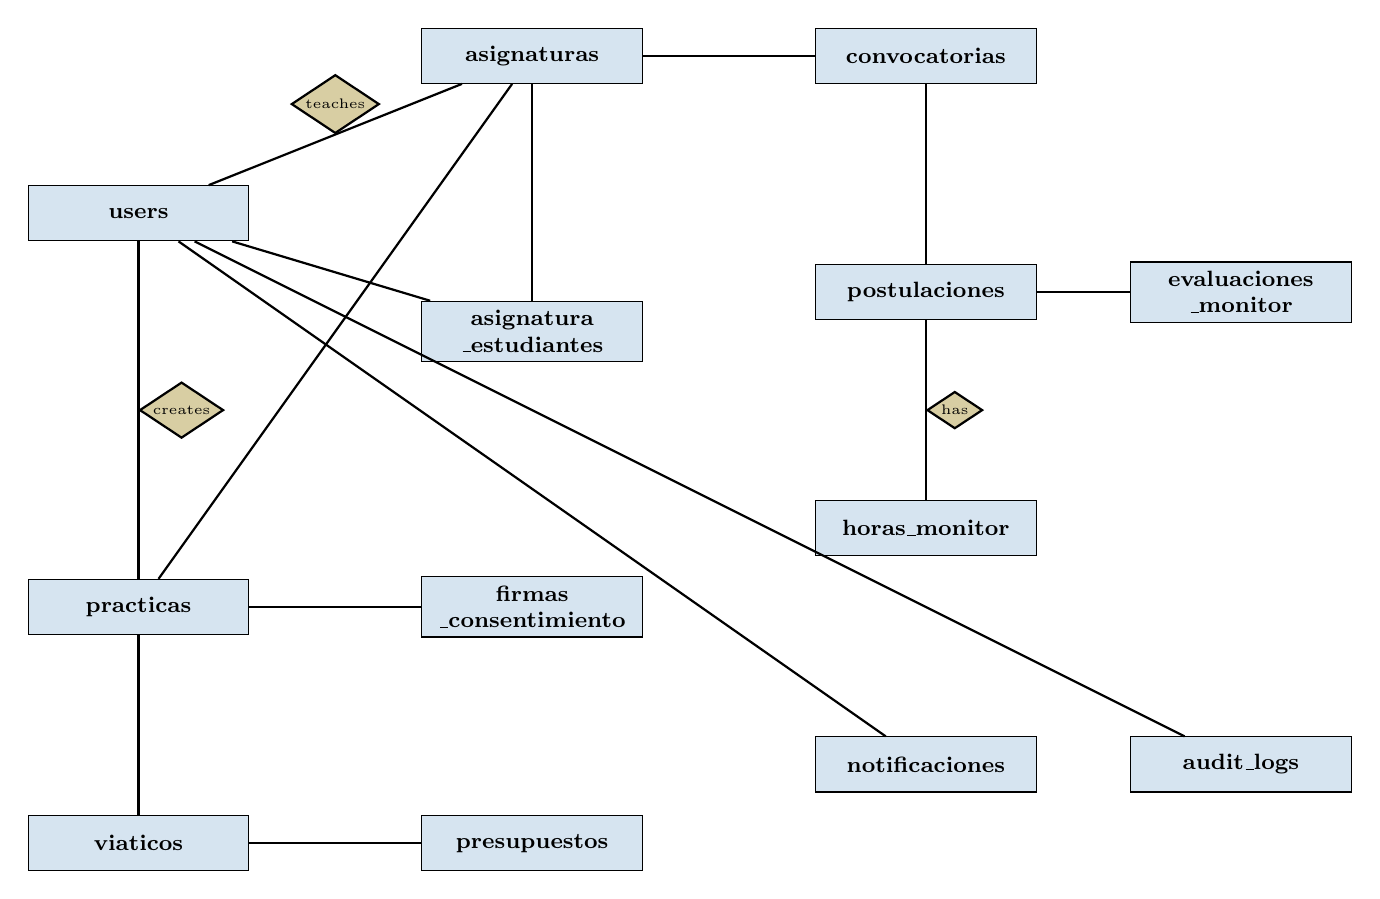
\begin{tikzpicture}[
  entity/.style={draw, rectangle, minimum width=2.8cm, minimum height=0.7cm,
                 fill=softblue, font=\footnotesize\bfseries, align=center},
  attr/.style={font=\tiny, color=grisusco},
  rel/.style={draw, diamond, aspect=1.5, fill=ocre, font=\tiny, inner sep=1pt},
  line/.style={-, thick},
  arr/.style={-, >=Latex}
]

  \node[entity] (users)      at (0,0)      {users};
  \node[entity] (asig)       at (5,2)      {asignaturas};
  \node[entity] (ae)         at (5,-1.5)   {asignatura\\\_estudiantes};
  \node[entity] (conv)       at (10,2)     {convocatorias};
  \node[entity] (post)       at (10,-1)    {postulaciones};
  \node[entity] (horas)      at (10,-4)    {horas\_monitor};
  \node[entity] (eval)       at (14,-1)    {evaluaciones\\\_monitor};
  \node[entity] (prac)       at (0,-5)     {practicas};
  \node[entity] (firmas)     at (5,-5)     {firmas\\\_consentimiento};
  \node[entity] (viaticos)   at (0,-8)     {viaticos};
  \node[entity] (presup)     at (5,-8)     {presupuestos};
  \node[entity] (notif)      at (10,-7)    {notificaciones};
  \node[entity] (audit)      at (14,-7)    {audit\_logs};

  % users relationships
  \draw[line] (users) -- node[rel,above]{teaches} (asig);
  \draw[line] (users) -- (ae);
  \draw[line] (users) -- node[rel,right]{creates} (prac);
  \draw[line] (users) -- (notif);
  \draw[line] (users) -- (audit);
  % asig
  \draw[line] (asig) -- (ae);
  \draw[line] (asig) -- (conv);
  \draw[line] (asig) -- (prac);
  % conv / post
  \draw[line] (conv) -- (post);
  \draw[line] (post) -- node[rel,right]{has} (horas);
  \draw[line] (post) -- (eval);
  % practicas
  \draw[line] (prac) -- (firmas);
  \draw[line] (prac) -- (viaticos);
  \draw[line] (presup) -- (viaticos);

\end{tikzpicture}
\end{center}

\vspace{0.5cm}
\noindent\textbf{Key relationships:}
\begin{itemize}[noitemsep]
  \item \textbf{users} (1) $\to$ (N) \textbf{asignaturas} — a professor teaches many subjects
  \item \textbf{users} (N) $\leftrightarrow$ (N) \textbf{asignaturas} via \textbf{asignatura\_estudiantes} — students enroll in subjects
  \item \textbf{convocatorias} (1) $\to$ (N) \textbf{postulaciones} — a vacancy has many applicants
  \item \textbf{postulaciones} (1) $\to$ (N) \textbf{horas\_monitor} — selected monitors log hours per week
  \item \textbf{practicas} (1) $\to$ (N) \textbf{firmas\_consentimiento} — a practice collects signatures
  \item \textbf{practicas} (1) $\to$ (N) \textbf{viaticos} — a practice has multiple per-diem line items
\end{itemize}

% ══════════════════════════════════════════════════════════════════════════════
\section{Class Diagrams}
% ══════════════════════════════════════════════════════════════════════════════

\subsection{Core Domain Models (SQLAlchemy)}

\begin{center}
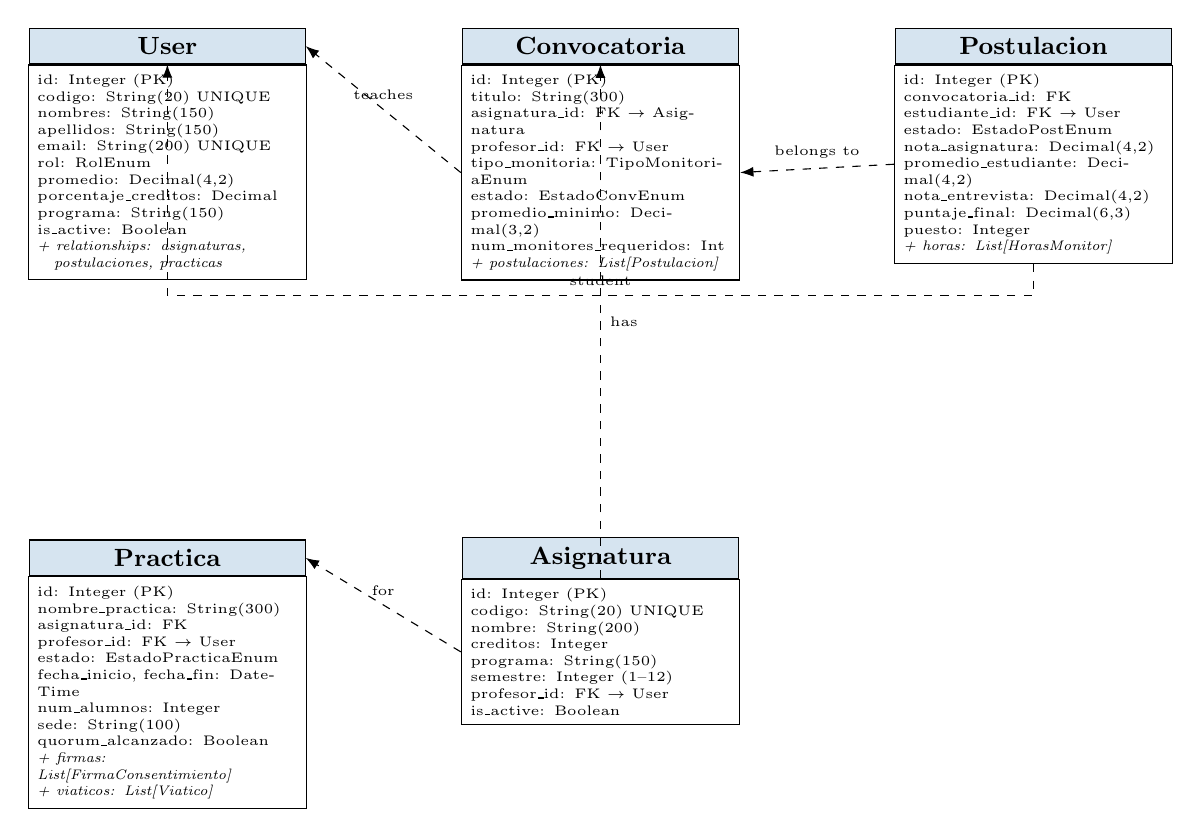
\begin{tikzpicture}[
  cls/.style={draw, rectangle, minimum width=3.5cm, font=\small},
  clstitle/.style={draw, rectangle, minimum width=3.5cm, fill=softblue, font=\small\bfseries},
  clsbody/.style={draw, rectangle, minimum width=3.5cm, font=\tiny, align=left, text width=3.3cm},
  inh/.style={->, >=open triangle 60, thick},
  assoc/.style={->, >=Latex, thin, dashed}
]

  % User class
  \node[clstitle]             (ut) at (0,0)     {User};
  \node[clsbody, below=0pt of ut] (ub) {
    id: Integer (PK)\\
    codigo: String(20) UNIQUE\\
    nombres: String(150)\\
    apellidos: String(150)\\
    email: String(200) UNIQUE\\
    rol: RolEnum\\
    promedio: Decimal(4,2)\\
    porcentaje\_creditos: Decimal\\
    programa: String(150)\\
    is\_active: Boolean\\
    \textit{+ relationships: asignaturas,}\\
    \textit{\quad postulaciones, practicas}
  };

  % Convocatoria class
  \node[clstitle]             (ct) at (5.5,0)    {Convocatoria};
  \node[clsbody, below=0pt of ct] (cb) {
    id: Integer (PK)\\
    titulo: String(300)\\
    asignatura\_id: FK $\to$ Asignatura\\
    profesor\_id: FK $\to$ User\\
    tipo\_monitoria: TipoMonitoriaEnum\\
    estado: EstadoConvEnum\\
    promedio\_minimo: Decimal(3,2)\\
    num\_monitores\_requeridos: Int\\
    \textit{+ postulaciones: List[Postulacion]}
  };

  % Postulacion class
  \node[clstitle]             (pt) at (11,0)    {Postulacion};
  \node[clsbody, below=0pt of pt] (pb) {
    id: Integer (PK)\\
    convocatoria\_id: FK\\
    estudiante\_id: FK $\to$ User\\
    estado: EstadoPostEnum\\
    nota\_asignatura: Decimal(4,2)\\
    promedio\_estudiante: Decimal(4,2)\\
    nota\_entrevista: Decimal(4,2)\\
    puntaje\_final: Decimal(6,3)\\
    puesto: Integer\\
    \textit{+ horas: List[HorasMonitor]}
  };

  % Practica class
  \node[clstitle]             (prt) at (0,-6.5)   {Practica};
  \node[clsbody, below=0pt of prt] (prb) {
    id: Integer (PK)\\
    nombre\_practica: String(300)\\
    asignatura\_id: FK\\
    profesor\_id: FK $\to$ User\\
    estado: EstadoPracticaEnum\\
    fecha\_inicio, fecha\_fin: DateTime\\
    num\_alumnos: Integer\\
    sede: String(100)\\
    quorum\_alcanzado: Boolean\\
    \textit{+ firmas: List[FirmaConsentimiento]}\\
    \textit{+ viaticos: List[Viatico]}
  };

  % Asignatura class
  \node[clstitle]             (at) at (5.5,-6.5)   {Asignatura};
  \node[clsbody, below=0pt of at] (ab) {
    id: Integer (PK)\\
    codigo: String(20) UNIQUE\\
    nombre: String(200)\\
    creditos: Integer\\
    programa: String(150)\\
    semestre: Integer (1–12)\\
    profesor\_id: FK $\to$ User\\
    is\_active: Boolean
  };

  \draw[assoc] (cb.west) -- (ut.east) node[midway,above,font=\tiny]{teaches};
  \draw[assoc] (pb.west) -- (cb.east) node[midway,above,font=\tiny]{belongs to};
  \draw[assoc] (pb.south) -- ++(0,-0.4) -| (ut.south) node[near start, above, font=\tiny]{student};
  \draw[assoc] (ab.north) -- (ct.south) node[midway, right, font=\tiny]{has};
  \draw[assoc] (ab.west) -- (prt.east) node[midway,above,font=\tiny]{for};

\end{tikzpicture}
\end{center}

% ══════════════════════════════════════════════════════════════════════════════
\section{GUI Design — Key Screens}
% ══════════════════════════════════════════════════════════════════════════════

The SIPAM-USCO frontend is a Single-Page Application (SPA) built with React 19, TypeScript,
and Tailwind CSS v4. Key screens include:

\begin{enumerate}
  \item \textbf{Login screen} — Institutional branding (vinotinto \#8D191D), code/ID + password authentication.
  \item \textbf{Dashboard} — Role-specific widgets showing pending actions, statistics, and notifications.
  \item \textbf{Tutoring panel} (professor) — Vacancy management, applicant list, grade entry, algorithm execution, and ranking visualization.
  \item \textbf{Application form} (student) — Subject selection, document upload, and AI prediction widget.
  \item \textbf{Field practice wizard} (professor) — Multi-step form: route builder with map, date picker, participants, FO-16 data, transport cost estimator.
  \item \textbf{Approval queue} (head/dean/admin) — Pending practices with approve/reject actions and full details sidebar.
  \item \textbf{Budget panel} (admin) — Bar charts showing committed vs.\ executed spending per period.
  \item \textbf{AI Predictor} — Input form (GPA, credits, subject grade, interview score) with prediction result card showing probability bar and recommendation.
\end{enumerate}

% ══════════════════════════════════════════════════════════════════════════════
\section{Web Services Catalog}
% ══════════════════════════════════════════════════════════════════════════════

\subsection{Main API (FastAPI) — Base URL: \texttt{/api/v1}}

\begin{longtable}{>{\ttfamily}p{1.4cm} >{\ttfamily}p{5.8cm} p{5.5cm}}
  \toprule
  \textbf{Method} & \textbf{Endpoint} & \textbf{Description} \\
  \midrule
  \endfirsthead \toprule \textbf{Method} & \textbf{Endpoint} & \textbf{Description} \\ \midrule \endhead
  POST & /auth/login & JWT login \\
  GET  & /auth/me & Current user info \\
  GET  & /convocatorias/ & List vacancies \\
  POST & /convocatorias/ & Create vacancy \\
  POST & /postulaciones/convocatoria/\{id\} & Apply to vacancy \\
  PATCH & /postulaciones/\{id\}/desistir & Withdraw application \\
  POST & /seleccion/convocatorias/\{id\}/ejecutar-seleccion & Run selection algorithm \\
  GET  & /seleccion/convocatorias/\{id\}/resultados & Get selection results \\
  POST & /practicas/ & Create field practice \\
  PATCH & /practicas/\{id\}/aprobar & Approve (stage-based) \\
  POST & /practicas/\{id\}/firmar-consentimiento & Sign consent \\
  GET  & /reportes/fo05/\{id\} & FO-05 data (PDF) \\
  GET  & /reportes/fo15/\{id\} & FO-15 data (PDF) \\
  POST & /ia/predecir & AI prediction proxy \\
  GET  & /notificaciones/ & List notifications \\
  GET  & /transporte/costos/\{id\} & Transport cost calc \\
  \bottomrule
\end{longtable}

\subsection{AI Microservice (Flask) — Base URL: \texttt{http://localhost:5001}}

\begin{longtable}{>{\ttfamily}p{1.4cm} >{\ttfamily}p{4cm} p{4cm} p{3cm}}
  \toprule
  \textbf{Method} & \textbf{Endpoint} & \textbf{Description} & \textbf{Body / Response} \\
  \midrule
  GET  & /health & Service health check & \texttt{\{"status":"ok"\}} \\
  POST & /predict & Predict selection outcome & Body: features JSON \\
  GET  & /models/metrics & Compare all 3 models & Accuracy, F1, AUC \\
  GET  & /models/feature-importance & Feature importances & Best model features \\
  \bottomrule
\end{longtable}

\noindent\textbf{Example request} to \ep{POST /predict}:
\begin{verbatim}
{
  "promedio": 4.1,
  "porcentaje_creditos": 65.0,
  "nota_asignatura": 4.5,
  "nota_entrevista": 4.2,
  "tipo_monitoria": "academica",
  "semestre_asignatura": 4,
  "creditos_asignatura": 3,
  "num_postulantes": 8,
  "num_monitores_requeridos": 2
}
\end{verbatim}

\noindent\textbf{Example response}:
\begin{verbatim}
{
  "selected_probability": 0.82,
  "prediction": "selected",
  "confidence": "high",
  "model_used": "XGBoost",
  "puntaje_estimado": 4.23,
  "rank_estimado": 1
}
\end{verbatim}

% ══════════════════════════════════════════════════════════════════════════════
\section{AI Model Architecture}
% ══════════════════════════════════════════════════════════════════════════════

\subsection{Problem Formulation}
\textbf{Task:} Binary classification — predict whether a student will be \textit{selected}
(1) or \textit{not selected} (0) as a tutoring monitor.

\textbf{Input features:}
\begin{center}
\begin{tabular}{llll}
  \toprule
  \textbf{Feature} & \textbf{Type} & \textbf{Range} & \textbf{Source} \\
  \midrule
  promedio & Continuous & 0.0 – 5.0 & users table \\
  porcentaje\_creditos & Continuous & 0 – 100 & users table \\
  nota\_asignatura & Continuous & 0.0 – 5.0 & postulaciones \\
  nota\_entrevista & Continuous & 0.0 – 5.0 & postulaciones \\
  tipo\_monitoria & Categorical & 13 types & convocatorias \\
  semestre\_asignatura & Ordinal & 1 – 12 & asignaturas \\
  creditos\_asignatura & Ordinal & 1 – 6 & asignaturas \\
  num\_postulantes & Integer & 1 – 50 & computed \\
  num\_monitores\_requeridos & Integer & 1 – 5 & convocatorias \\
  \bottomrule
\end{tabular}
\end{center}

\textbf{Target:} \texttt{seleccionado} $\in \{0, 1\}$

\subsection{Pipeline Architecture}

\begin{center}
\begin{tikzpicture}[
  box/.style={draw, rectangle, rounded corners=4pt, minimum width=2.8cm,
              minimum height=0.8cm, align=center, font=\small},
  data/.style={box, fill=softblue},
  proc/.style={box, fill=softyellow},
  model/.style={box, fill=softgreen},
  out/.style={box, fill=ocre},
  arr/.style={->, >=Latex, thick}
]
  \node[data]  (db)     at (0,0)       {PostgreSQL\\sipam\_db};
  \node[proc]  (ext)    at (3.5,0)     {extract\_\\dataset.py};
  \node[proc]  (prep)   at (7,0)       {prepare\_\\dataset.py};
  \node[proc]  (split)  at (10.5,0)    {70/15/15\\Split};

  \node[model] (rf)     at (3.5,-2.5)  {Random\\Forest};
  \node[model] (xgb)    at (7,-2.5)    {XGBoost};
  \node[model] (nn)     at (10.5,-2.5) {Neural Net\\(TensorFlow)};

  \node[proc]  (eval)   at (7,-4.5)    {Metrics:\\Acc · F1 · AUC};
  \node[model] (best)   at (7,-6.5)    {Best Model\\(.joblib / .h5)};
  \node[out]   (flask)  at (7,-8.5)    {Flask API\\POST /predict};
  \node[out]   (react)  at (7,-10.5)   {React UI\\Prediction Widget};

  \draw[arr] (db) -- (ext);
  \draw[arr] (ext) -- (prep);
  \draw[arr] (prep) -- (split);
  \draw[arr] (split) -- ++(0,-1.2) -| (rf);
  \draw[arr] (split) -- ++(0,-1.2) -| (xgb);
  \draw[arr] (split) -- (nn);
  \draw[arr] (rf) -- (eval);
  \draw[arr] (xgb) -- (eval);
  \draw[arr] (nn) -- (eval);
  \draw[arr] (eval) -- node[right,font=\small]{serialize} (best);
  \draw[arr] (best) -- node[right,font=\small]{load} (flask);
  \draw[arr] (flask) -- node[right,font=\small]{REST} (react);
\end{tikzpicture}
\end{center}

\subsection{Models Compared}
\begin{center}
\begin{tabular}{llll}
  \toprule
  \textbf{Model} & \textbf{Library} & \textbf{Hyperparameters} & \textbf{Tuning} \\
  \midrule
  Random Forest     & scikit-learn & n\_estimators=300, max\_depth=10 & GridSearchCV \\
  XGBoost           & xgboost      & n\_estimators=200, lr=0.05       & GridSearchCV \\
  Neural Network    & TensorFlow   & Dense(64→32→1), dropout=0.3      & Hyperband \\
  \bottomrule
\end{tabular}
\end{center}

\subsection{Data Split Strategy}
\begin{center}
\begin{tabular}{lcl}
  \toprule
  \textbf{Partition} & \textbf{Size} & \textbf{Purpose} \\
  \midrule
  Training set   & 70\% & Model fitting \\
  Validation set & 15\% & Hyperparameter tuning \\
  Test set       & 15\% & Final unbiased evaluation \\
  \bottomrule
\end{tabular}
\end{center}

\noindent Stratified splitting is used to preserve class distribution across all partitions.
Class imbalance (if present) is handled with SMOTE on the training partition only.

% ══════════════════════════════════════════════════════════════════════════════
\section{Test Cases}
% ══════════════════════════════════════════════════════════════════════════════

\subsection{Unit Tests — Flask AI Service}
\begin{longtable}{>{\bfseries}p{1.3cm} p{5cm} p{6cm}}
  \toprule
  \textbf{ID} & \textbf{Description} & \textbf{Expected Result} \\
  \midrule
  \endfirsthead \toprule \textbf{ID} & \textbf{Description} & \textbf{Expected Result} \\ \midrule \endhead
  UT-01 & \ep{POST /predict} with valid input & HTTP 200, \texttt{selected\_probability} in [0,1] \\
  UT-02 & \ep{POST /predict} with missing field & HTTP 422, field name in error detail \\
  UT-03 & \ep{POST /predict} with invalid promedio=6 & HTTP 422, validation error \\
  UT-04 & \ep{GET /models/metrics} & HTTP 200, 3 model entries with accuracy, F1, AUC \\
  UT-05 & Model file missing at startup & HTTP 503 with meaningful error \\
  UT-06 & Student with promedio=5.0 all features max & Probability $\geq$ 0.9 \\
  UT-07 & Student with promedio=3.5 all features min & Probability $\leq$ 0.4 \\
  \bottomrule
\end{longtable}

\subsection{Functional Tests — Full Pipeline}
\begin{longtable}{>{\bfseries}p{1.3cm} p{5cm} p{6cm}}
  \toprule
  \textbf{ID} & \textbf{Description} & \textbf{Expected Result} \\
  \midrule
  FT-01 & Student applies and sees AI prediction & Frontend renders probability bar with value \\
  FT-02 & Professor runs selection algorithm on 10 candidates & 3 selected, 7 not selected, puntajes match formula \\
  FT-03 & Field practice approval full flow & Practice transitions through all 3 stages \\
  FT-04 & Consent reaches 66\% $\to$ auto-advance & Practice state changes automatically \\
  FT-05 & Budget commitment on practice approval & Committed amount increases in presupuesto \\
  \bottomrule
\end{longtable}

\subsection{Integration Tests}
\begin{longtable}{>{\bfseries}p{1.3cm} p{5cm} p{6cm}}
  \toprule
  \textbf{ID} & \textbf{Description} & \textbf{Expected Result} \\
  \midrule
  IT-01 & React $\to$ FastAPI $\to$ Flask $\to$ Response & JSON prediction reaches React within 2s \\
  IT-02 & DB-backed brute force: 5 failed logins & 6th attempt returns HTTP 429 \\
  IT-03 & Flask reads student data from PostgreSQL & Query returns correct academic profile \\
  \bottomrule
\end{longtable}

% ══════════════════════════════════════════════════════════════════════════════
\section{Results and Discussion}
% ══════════════════════════════════════════════════════════════════════════════

\subsection{System Metrics}
\begin{center}
\begin{tabular}{lr}
  \toprule
  \textbf{Metric} & \textbf{Value} \\
  \midrule
  Total registered users    & 655 \\
  Academic subjects         & 51 \\
  Student enrollments       & 1,262 \\
  API endpoints implemented & $\approx$75 \\
  PDF forms generated       & 7 (FO-05, FO-14, FO-15, FO-15C, FO-16, FO-46, Consent) \\
  DB tables                 & 26 \\
  DB CHECK constraints      & 30+ \\
  DB indexes                & 42 \\
  \bottomrule
\end{tabular}
\end{center}

\subsection{Discussion}
The system successfully automates all paper-based processes previously handled manually at the
Faculty of Engineering. Key outcomes include:

\begin{itemize}
  \item \textbf{Regulatory compliance:} All business rules from Acuerdo 003/2012 and
        Acuerdo 012/2023 are enforced at the API level with CHECK constraints as a
        second line of defense.
  \item \textbf{Scalability:} The DB-backed brute-force protection and multi-worker-safe
        architecture allow horizontal scaling.
  \item \textbf{AI Integration:} The Flask microservice decouples the ML inference from the
        main FastAPI application, following the \textit{separation of concerns} principle.
  \item \textbf{Data integrity:} Moving from manual entry to a structured system with
        validation eliminates the inconsistencies present in the previous process.
\end{itemize}

% ══════════════════════════════════════════════════════════════════════════════
\section{Recommendations and Future Work}
% ══════════════════════════════════════════════════════════════════════════════

\begin{enumerate}
  \item \textbf{Real training data:} Once the system accumulates real postulation records
        (at least 2 academic periods), retrain the model on real data and compare with the
        synthetic baseline.
  \item \textbf{Model drift monitoring:} Implement a monitoring pipeline (e.g., Evidently AI)
        to detect concept drift as student demographics evolve.
  \item \textbf{Mobile app:} Develop a React Native companion app for students to sign consent
        forms and check application status on mobile.
  \item \textbf{IoT integration:} Install environmental sensors (temperature, humidity) in
        greenhouses used for field practices, feeding data to the system for practice planning.
  \item \textbf{External federation:} Integrate with the USCO academic registry API to
        auto-update student GPA and credit data rather than relying on manual seed data.
  \item \textbf{Cloud deployment:} Migrate to AWS/GCP with container orchestration (Docker +
        ECS or Cloud Run) for high-availability production deployment.
  \item \textbf{Federated learning:} Apply federated learning techniques (Topic 10 of this
        course) to train the AI model across multiple faculties without centralizing data.
\end{enumerate}

% ─────────────────────────────────────────────────────────────────────────────
\vfill
\begin{center}
  {\color{vinotinto}\rule{0.5\linewidth}{0.8pt}}\\[0.3cm]
  {\small Universidad Surcolombiana — Faculty of Engineering — Software Engineering}\\
  {\small SIPAM-USCO v1.0 — AI Course BEINSOF52 — May 2026}
\end{center}

\end{document}
